%%% Compile this example with xelatex! %%%
\documentclass{report}
\usepackage[utf8]{inputenc}
\usepackage{pgfpages}
\pgfpagesuselayout{2 on 1}[physical paper height=20cm, physical paper width=50cm, border shrink=-0mm]
\usepackage
[
        left=-3cm,
        right=-3cm,
        top=3cm,
        bottom=3.5cm
]
{geometry}
\usepackage[fontsize=28pt]{fontsize}  % define global font size here
\usepackage{fontspec}
\setmainfont{Liberation Serif}
\usepackage{graphicx}
\usepackage{hyperref}
\usepackage[center]{titlesec}
\titleformat{\section}
{\fontsize{60}{60}\bfseries}{\thesection}{0cm}{\rule{7cm}{2pt}\hspace{1cm}}
\setlength\parindent{0pt}

%%% Defining section command. Usage: \LPLsection{<Title>} %%%
\newcommand\pagetitle{SectionTitle}
\newcommand{\LPLsection}[1]{%
\begin{figure}%
    \centering%
    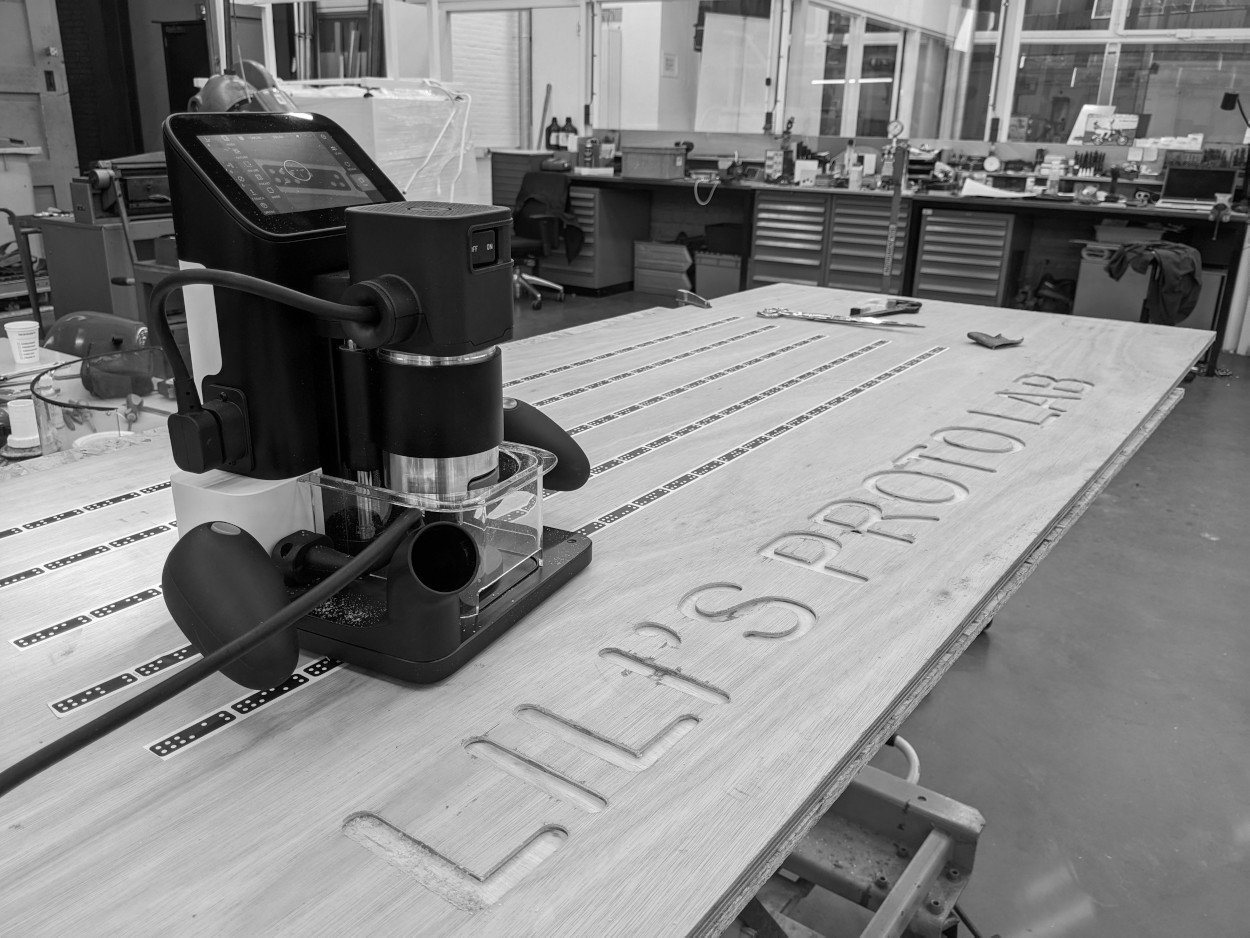
\includegraphics[height=\textheight]{design_images/LPL_shaper.jpg}%
\end{figure}%
\clearpage%
\,\vspace{\textheight/3}%
%\newcommand\pagetitle{#1}
\renewcommand\pagetitle{#1}% 
\section*{\centering \pagetitle}%
\addcontentsline{toc}{section}{\protect\numberline{}\pagetitle}%
\clearpage%
}
%%%%%%%%%%%%%%%%%%%%%%%%%%%%%%%%%%%%%%%%%%%%%%%%%%%%%%%%%%%%%%

\title{\fontsize{60}{60}\bfseries Yearly Report 2022}
\author{\fontsize{80}{80}\bfseries Lili's Proto Lab}
\date{Utrecht University, December 2022}

\begin{document}

\maketitle
\thispagestyle{empty}

\begin{figure}
    \centering
    
\includegraphics[height=\textheight]{design_images/neon_L.jpg}
\end{figure}
\clearpage

%%% Table of contents double page %%%%
\begin{figure}
    \centering
    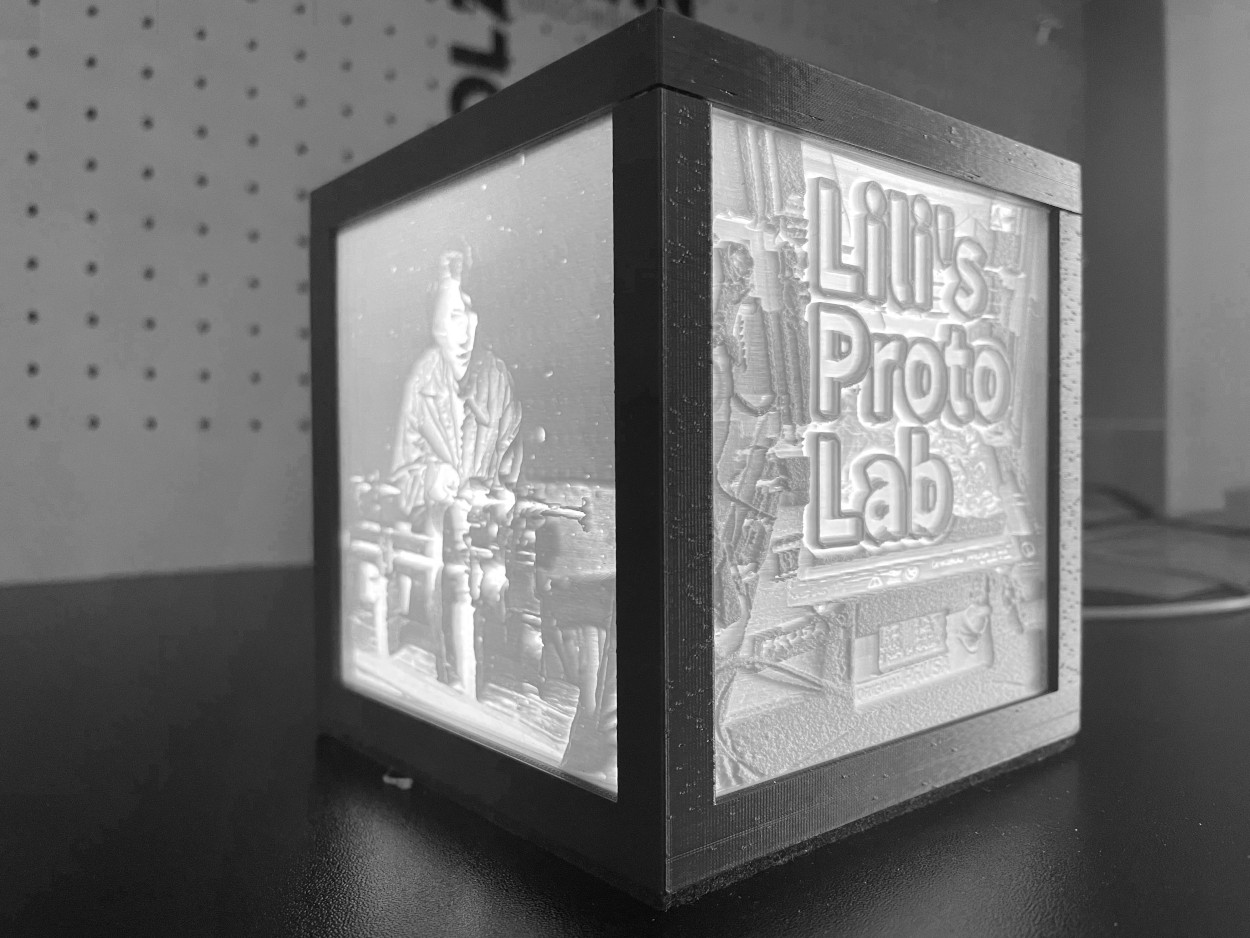
\includegraphics[height=\textheight]{design_images/cube.jpg}
\end{figure}
\pagenumbering{arabic}  % start page number 1 here
\clearpage
\tableofcontents
\clearpage
%%%%%%%%%%%%%%%%%%%%%%%%%%%%%%%%%%%%%%


\LPLsection{Introduction}

%%%%%%%%% New content page %%%%%%%%%%%
%%% Bold comment %%%
\noindent {\large \textbf{From an idea to success}} \\
%%%%%%%%%%%%%%%%%%%%

Welcome to the first annual report for Lili's Proto Lab! We are excited to share with you the progress and accomplishments of our maker space and prototyping lab over the past year. 2022 marked the first full year of operation for Lili's Proto Lab, and we are thrilled to have provided a space for the first UU students to explore their creativity and bring their ideas to life.

Throughout the year, our team has worked hard to create a welcoming and inclusive environment for all students to learn, create, and collaborate. We have doubled our team size from our supervisor board (consisting of Pauline Krijgsheld, Lennart Herlaar, and Sanli Faez) to a total of six with Pieter Kooijman (lab manager), Edward Paddon (project acquisition and development), and Jacob Seifert (Ph.D. student teaching assistant). \\

In this annual report, we will highlight some of the most impressive projects created by our students, as well as share some of the ways in which Lili's Proto Lab has grown and evolved over the past year. Furthermore, we want to illuminate the first events, workshops and meeting that were held at LPL. After our location has been renovated in early January 2023, we will continue and develop our activities further. We hope that this report will give you a sense of the potential that exists within our maker space and prototyping lab, and that it will inspire you to continue supporting and celebrating the creative and scientific work of our students. 

\clearpage
%%%%%%%%%%%%%%% end %%%%%%%%%%%%%%%%%%

%%%%%%%%% New section page %%%%%%%%%%%
\begin{figure}
    \centering
    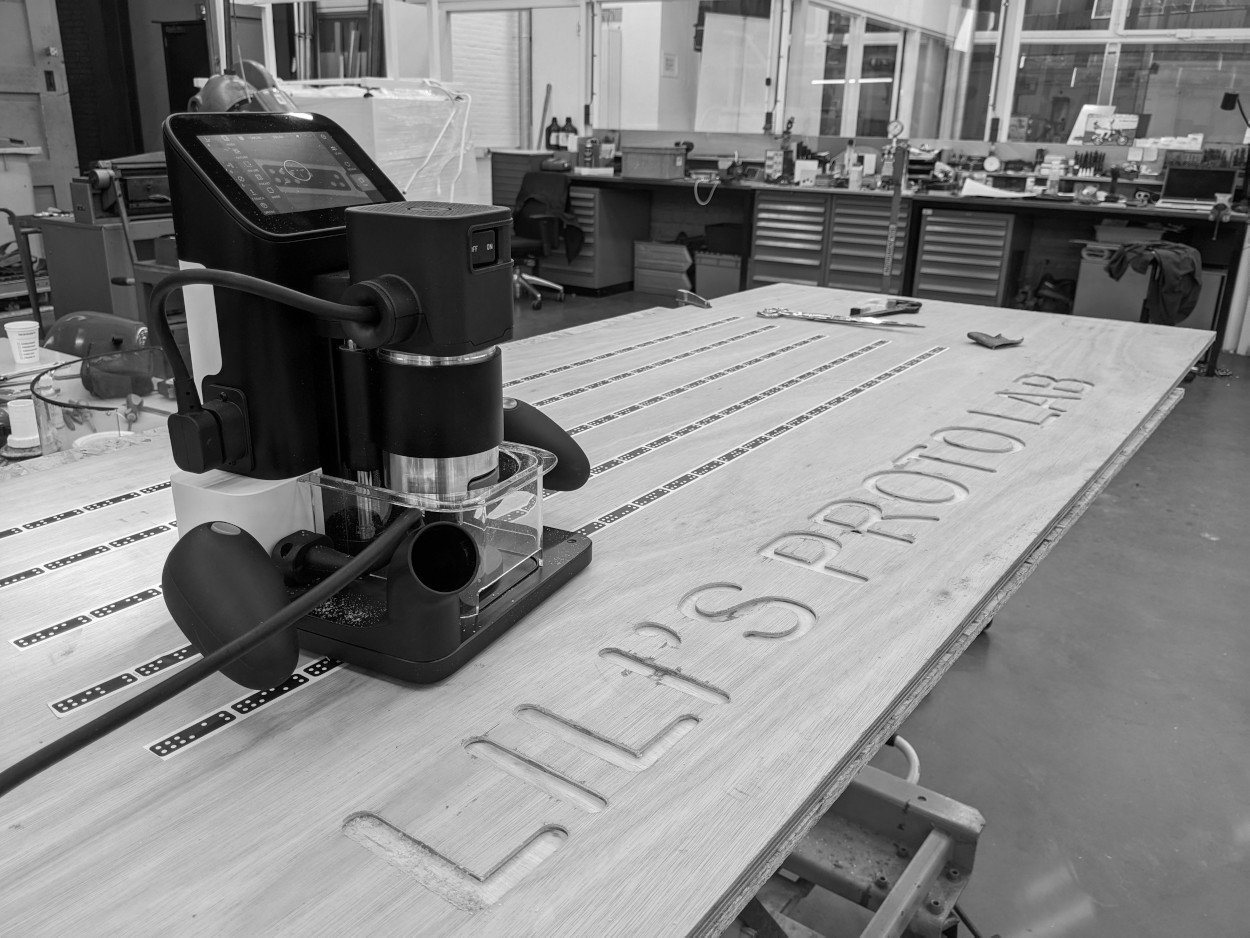
\includegraphics[height=\textheight]{design_images/LPL_shaper.jpg}
\end{figure}
\clearpage
\,\vspace{\textheight/3}
\renewcommand\pagetitle{Overview}   % section title
\section*{\centering \pagetitle}
\addcontentsline{toc}{section}{\protect\numberline{}\pagetitle}
\clearpage
%%%%%%%%%%%%%%%%%%%%%%%%%%%%%%%%%%%%%%%

%%%%%%%%% New content page %%%%%%%%%%%
%%% Bold comment %%%
\noindent {\large \textbf{We found a home in Caroline Bleeker Building}} \\
%%%%%%%%%%%%%%%%%%%%

At the beginning of 2022, finding an ideal space for the prototyping lab took us a while. We are happy to have found a home in Caroline Bleeker Building next to the Jobshop and Scientific Instrumentation [1]. The location provided us with the inspiration for our name: Caroline's nickname used to be Lili. Her path as an entrepreneur, business owner, consultant, and instrument maker can serve as an inspiration for our students.

By clicking the link below, you can now also find us on Maps [2].\\

[1] \url{https://www.uu.nl/en/research/scientific-instrumentation/the-job-shop}\\

[2] \url{https://goo.gl/maps/3gFvw4MbDppLuKGa8}

\clearpage
\begin{figure}
    \centering
    \makebox[\textwidth]{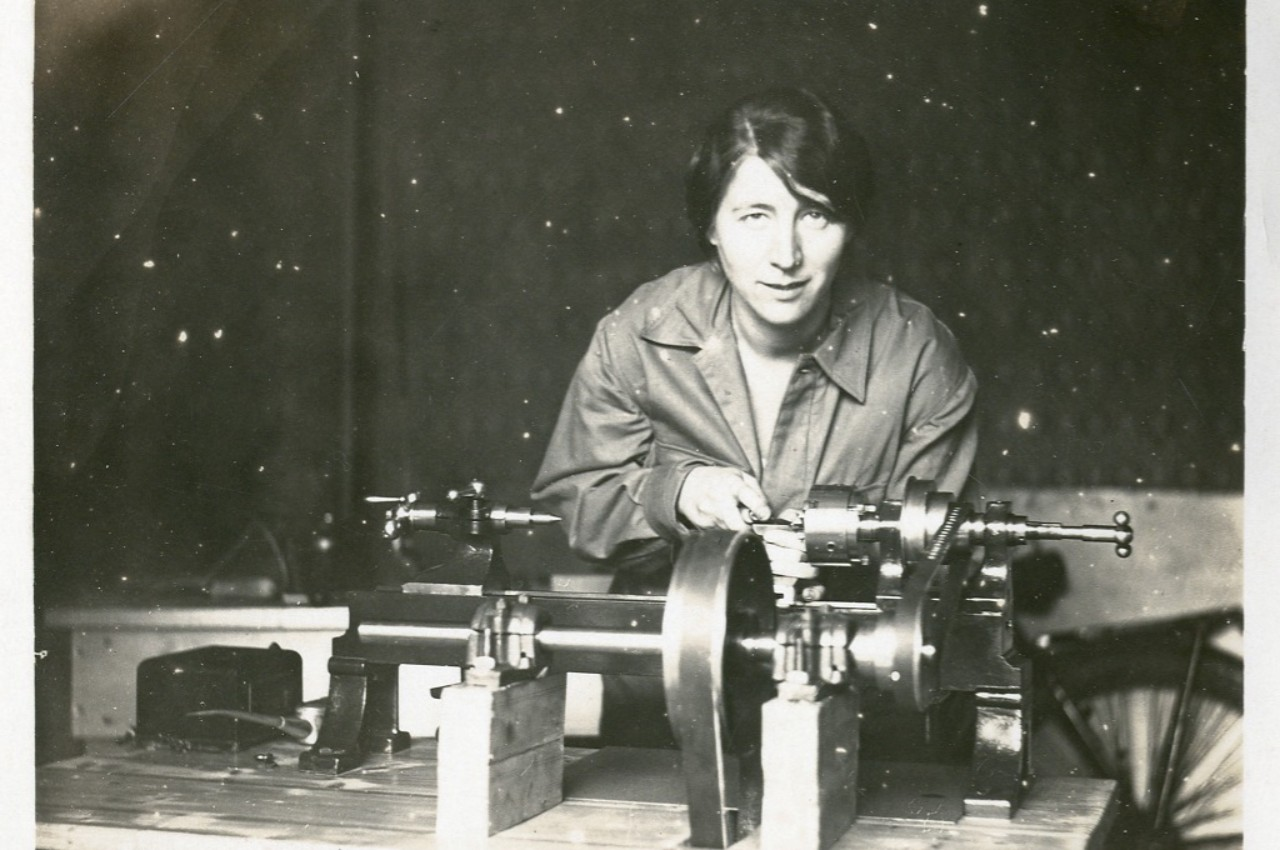
\includegraphics[height=\textheight]{images/bleeker.jpg}}
\end{figure}
\clearpage
%%%%%%%%%%%%%%% end %%%%%%%%%%%%%%%%%%


%%%%%%%%% New content page %%%%%%%%%%%
%%% Bold comment %%%
\noindent {\large \textbf{2022 closes with a construction and remodeling phase}} \\
%%%%%%%%%%%%%%%%%%%%

Lili's Proto Lab will be remodeled and modernized in Winter 2022/23. As a result, we had to pack up most of our equipment and temporarily store it in boxes. The grand opening day of LPL will be \textbf{March 8th, 2022}. Until then, our laser cutter and 3D printers remain operational in nearby rooms. 

\clearpage
\begin{figure}
    \centering
    \makebox[\textwidth]{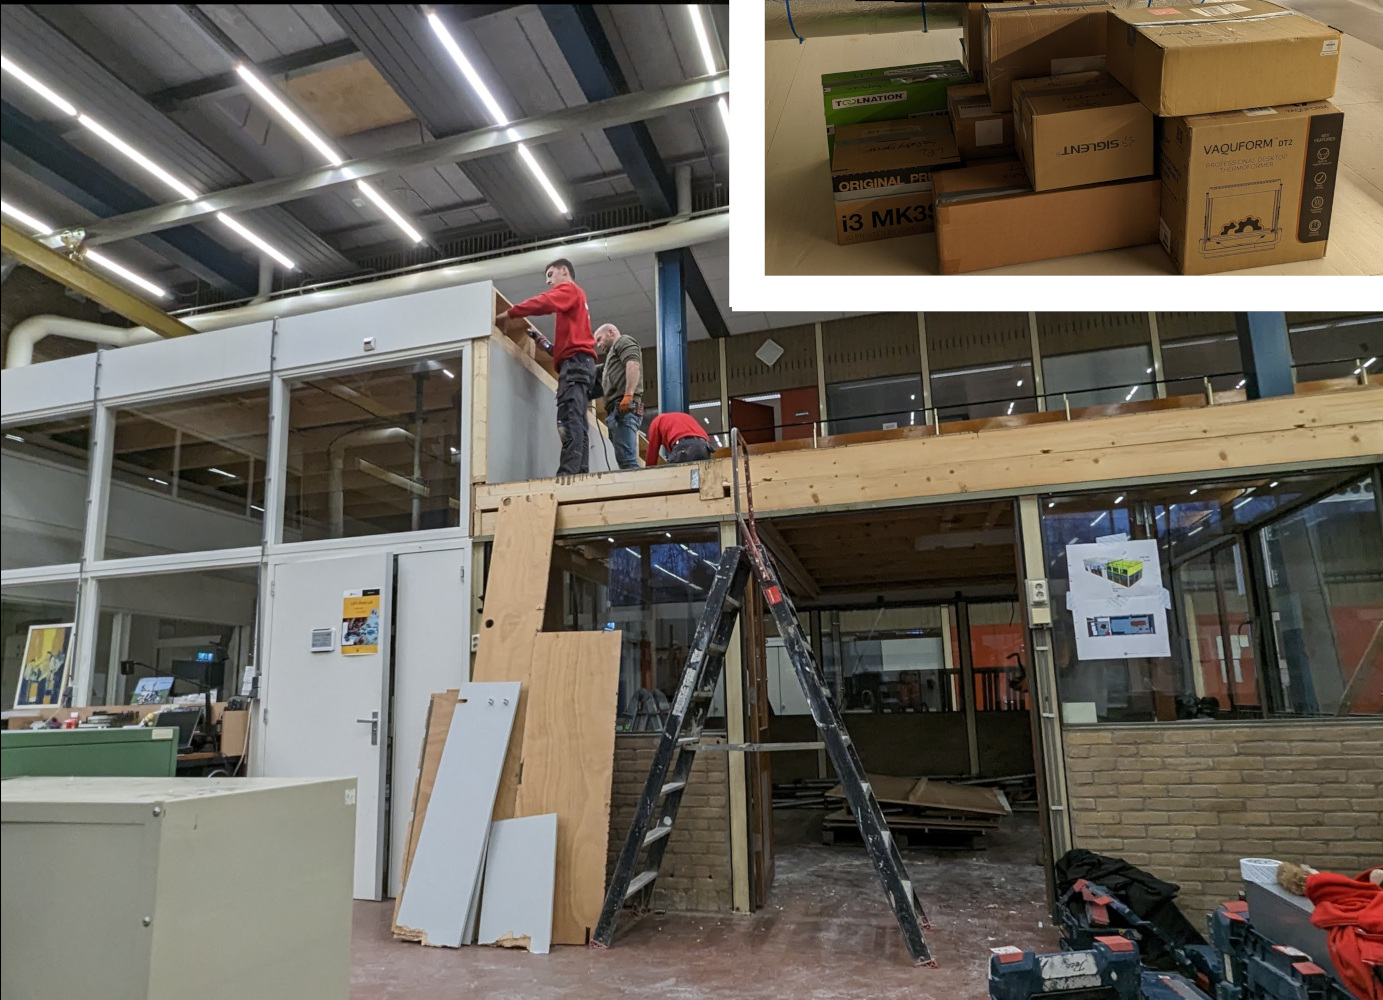
\includegraphics[height=\textheight]{images/remodeling.jpg}}
\end{figure}
\clearpage
%%%%%%%%%%%%%%% end %%%%%%%%%%%%%%%%%%

%%%%%%%%% New content page %%%%%%%%%%%
%%% Bold comment %%%
\noindent {\large \textbf{Our presence on the web}} \\
%%%%%%%%%%%%%%%%%%%%

Our new web presence is helping us be discoverable from within and outside the university. Our website serves as a central hub about LPL, including our mission, activities, and events [1]. We have a JOGL account to connect with other makers and share updates and resources [2]. In addition, we have a Twitter handle to share news and updates with a broader audience [3]. We also have a GitHub page showcasing our open-source projects and allowing others to contribute to our work [4]. Finally, we have a Mailman newsletter [5]. Overall, these web presences help us connect with our community and share our work with a broader audience. \\

[1] \url{https://www.uu.nl/LPL}

[2] \url{https://app.jogl.io/space/lpl}

[3] \url{https://twitter.com/LilisProtoLab}

[4] \url{https://github.com/LilisProtoLab}

[5] \url{https://mailman.science.uu.nl/mailman/listinfo/lpl-news}

\clearpage
\begin{figure}
    \centering
    \makebox[\textwidth]{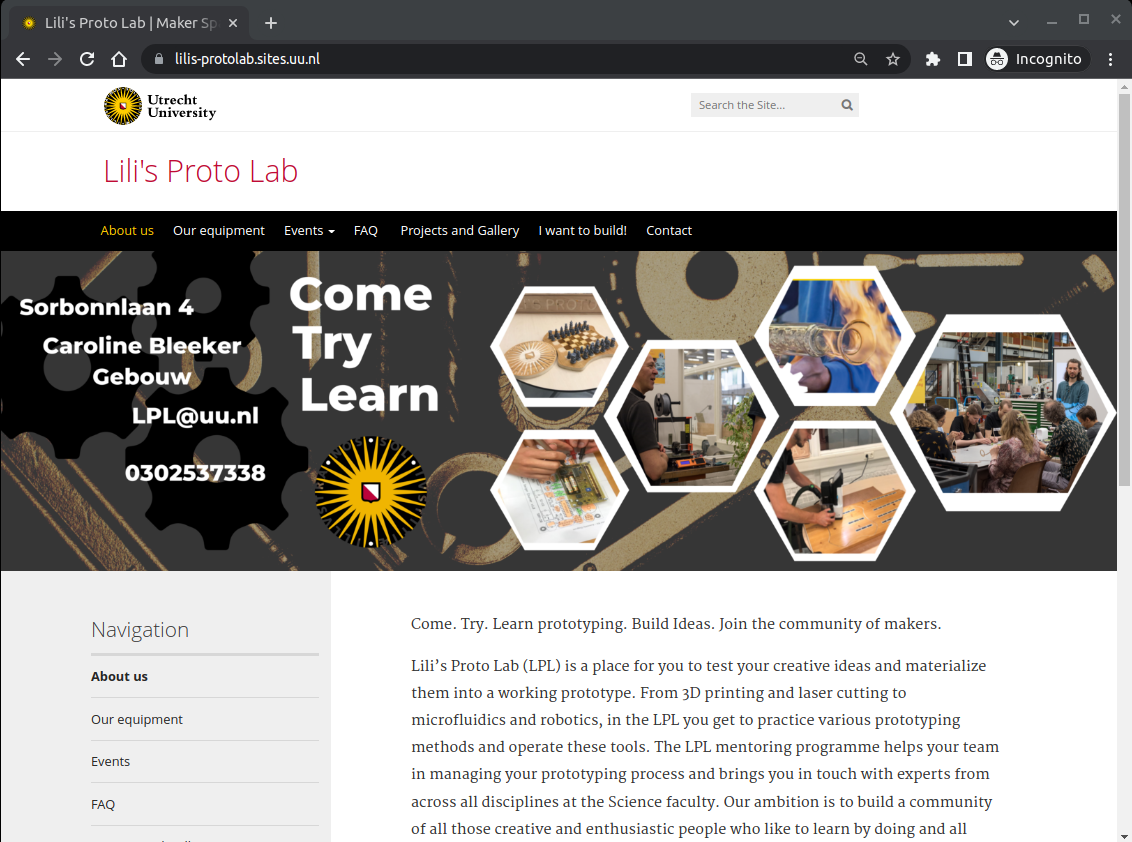
\includegraphics[height=\textheight]{images/LPL_website.png}}
\end{figure}
\clearpage
%%%%%%%%%%%%%%% end %%%%%%%%%%%%%%%%%%


\LPLsection{Members}

%%%%%%%%% New content page %%%%%%%%%%%
%%% Bold comment %%%
\noindent {\large \textbf{Our team has materialized...}} \\
%%%%%%%%%%%%%%%%%%%%

... and is comprised of three scientific staff members, two post-graduate coordinators, and a full-time lab manager.

\clearpage
\begin{figure}
    \centering
    \makebox[\textwidth]{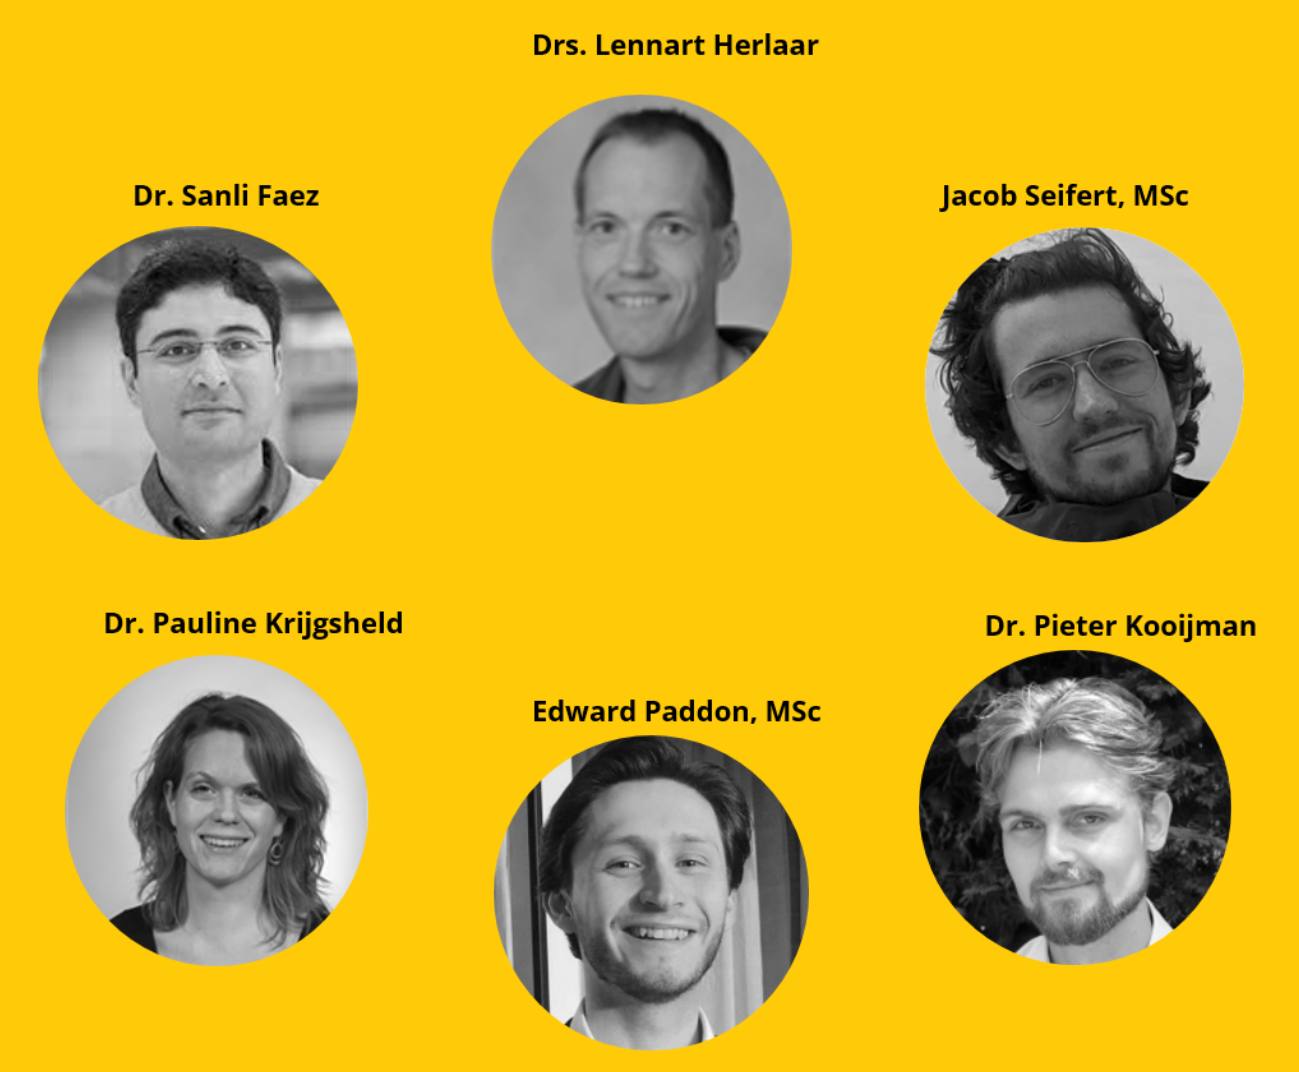
\includegraphics[height=\textheight]{images/members.png}}
\end{figure}
\clearpage
%%%%%%%%%%%%%%% end %%%%%%%%%%%%%%%%%%

\LPLsection{Events}

%%%%%%%%% New content page %%%%%%%%%%%
%%% Bold comment %%%
\noindent {\large \textbf{Faculty Day workshop}} \\
%%%%%%%%%%%%%%%%%%%%

We hosted a Faculty Day workshop on July 5th using one of our first tools: the laser cutter. All workshop participants were invited to laser-cut a silhouette vase from plywood. We had more than 20 participants in total and just that many keepsakes in form of those stylish vases that could be taken home. 

\clearpage
\begin{figure}
    \centering
    \makebox[\textwidth]{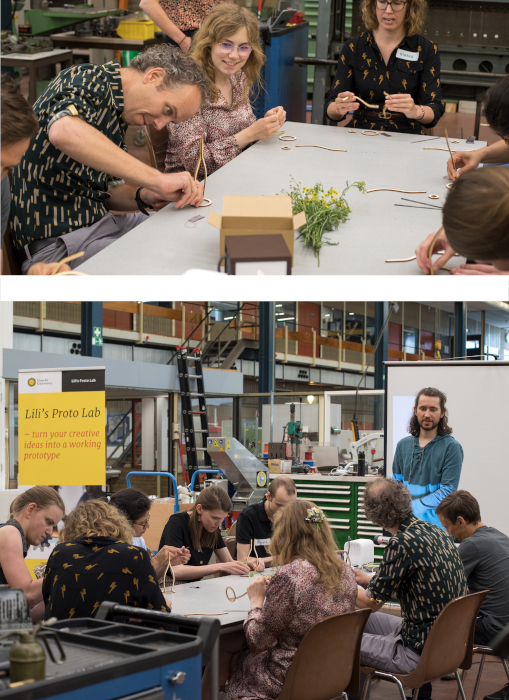
\includegraphics[height=\textheight]{images/facultyDay.jpg}}
\end{figure}
\clearpage
%%%%%%%%%%%%%%% end %%%%%%%%%%%%%%%%%%%

%%%%%%%%% New content page %%%%%%%%%%%
%%% Bold comment %%%
\noindent {\large \textbf{Advisory Board Meeting}} \\
%%%%%%%%%%%%%%%%%%%%

In November 2022, we celebrated our first advisory board meeting. The board consists of employees and students of Utrecht University, and will help us align and realize our teaching and outreach goals. At the first meeting, we were discussing relatively broad strategic questions such as community building, teaching, and how to orchestrate an interdisciplinary lab that needs to connect with all departments. Our next meeting is scheduled for Spring 2023.

\clearpage
\begin{figure}
    \centering
    \makebox[\textwidth]{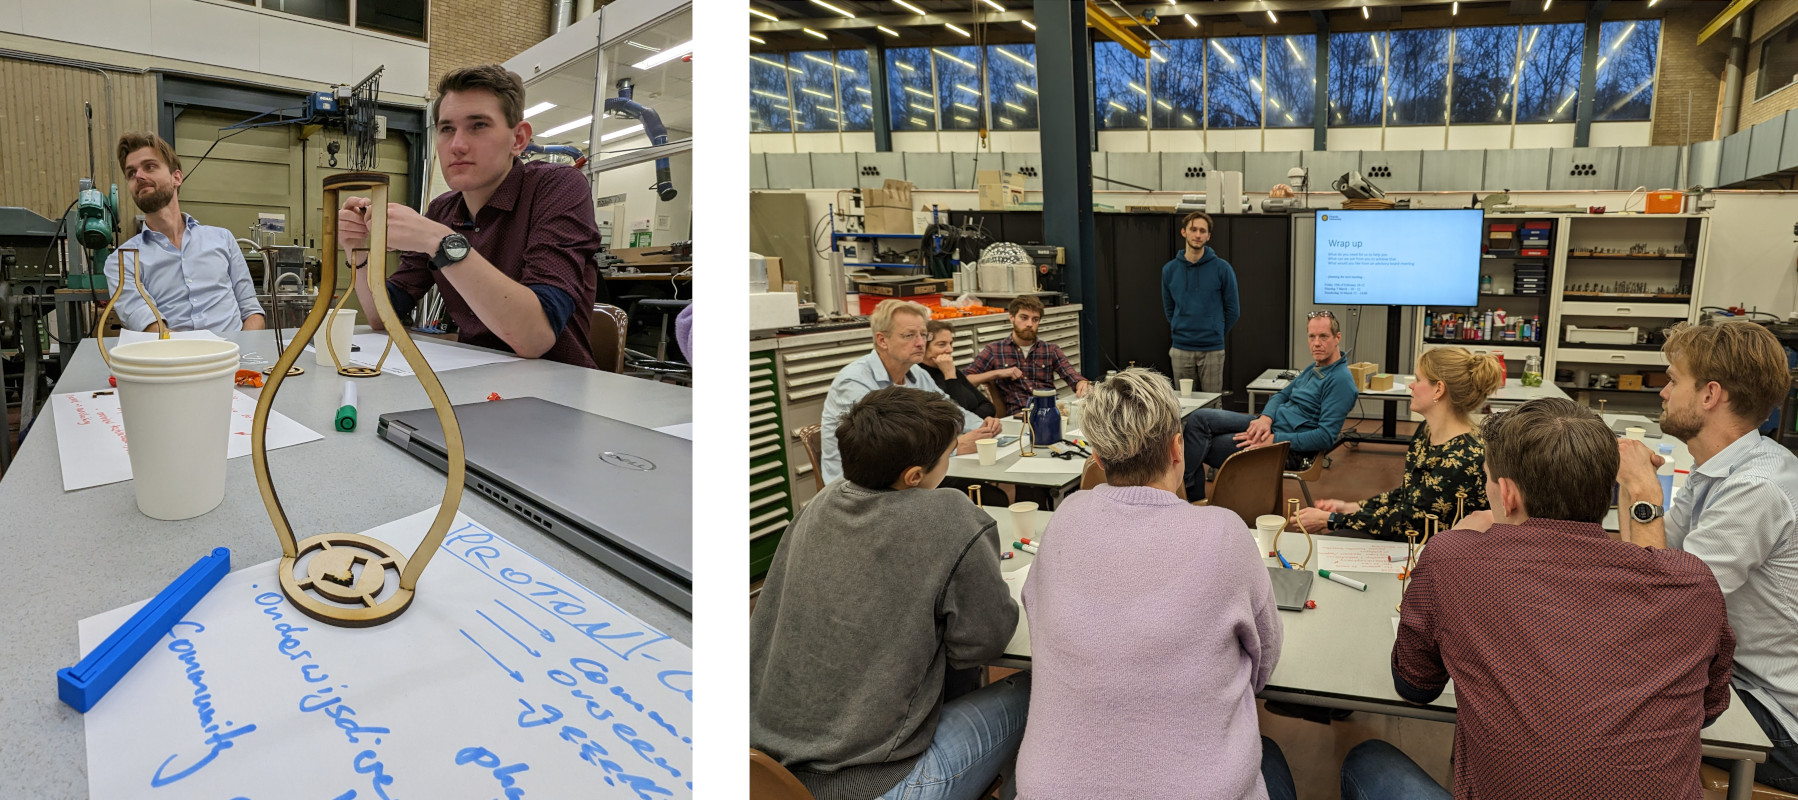
\includegraphics[height=0.8\textheight]{images/advisory_meeting.jpg}}
\end{figure}
\clearpage
%%%%%%%%%%%%%%% end %%%%%%%%%%%%%%%%%%%

%%%%%%%%% New content page %%%%%%%%%%%
%%% Bold comment %%%
\noindent {\large \textbf{Celebrating the Experimental Design course}} \\
%%%%%%%%%%%%%%%%%%%%

Also, in November 2022, the final presentations and demos of the course Experimental Design were held in Minnaertgebouw. We were impressed to see the creativity of the groups of students who built working prototypes quickly.  \\

In this course, students team up to build a hardware project with a research goal in mind. They need to build their setups from scratch in a short time of about four weeks. The Proto lab has been instrumental in making such rapid development possible. This year, a total of six experimental projects were realized.
Executing these projects is an opportunity for the student to learn how to contribute to open and collaborative experimental research and enhance their interpersonal skills. \\ 

One successful project was \textbf{LiPaTrap}: a linear particle trap that is documented on \url{https://app.jogl.io/project/1508/LiPaTrap}


\clearpage
\begin{figure}
    \centering
    \makebox[\textwidth]{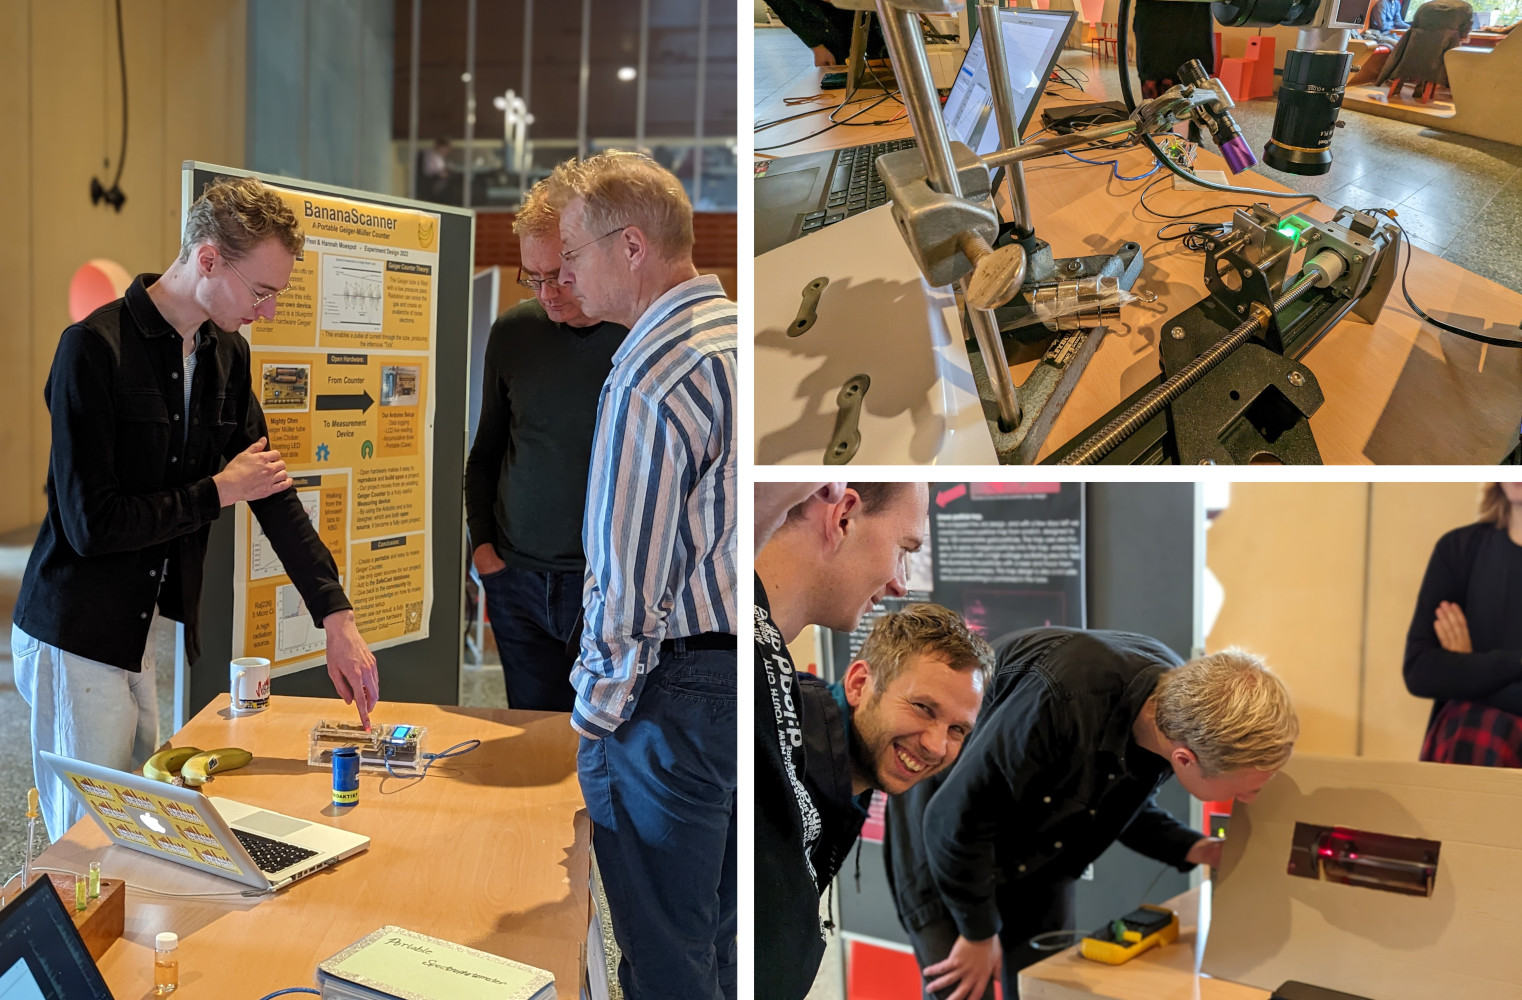
\includegraphics[height=\textheight]{images/ed_presentations.jpg}}
\end{figure}
\clearpage
%%%%%%%%%%%%%%% end %%%%%%%%%%%%%%%%%%%

%%%%%%%%% New content page %%%%%%%%%%%
%%% Bold comment %%%
\noindent {\large \textbf{PAULINE courses}} \\
%%%%%%%%%%%%%%%%%%%%

Brief description of the physics courses at LPL (even if only in planning phase so far)

\clearpage
\begin{figure}
    \centering
    \makebox[\textwidth]{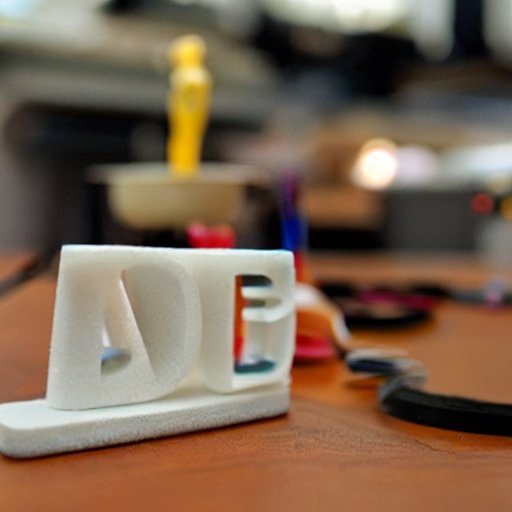
\includegraphics[height=\textheight]{images/replace_me.jpg}}
\end{figure}
\clearpage
%%%%%%%%%%%%%%% end %%%%%%%%%%%%%%%%%%

%%%%%%%%% New content page %%%%%%%%%%%
%%% Bold comment %%%
\noindent {\large \textbf{LENNART courses}} \\
%%%%%%%%%%%%%%%%%%%%

Brief description of the physics courses at LPL (even if only in planning phase so far)

\clearpage
\begin{figure}
    \centering
    \makebox[\textwidth]{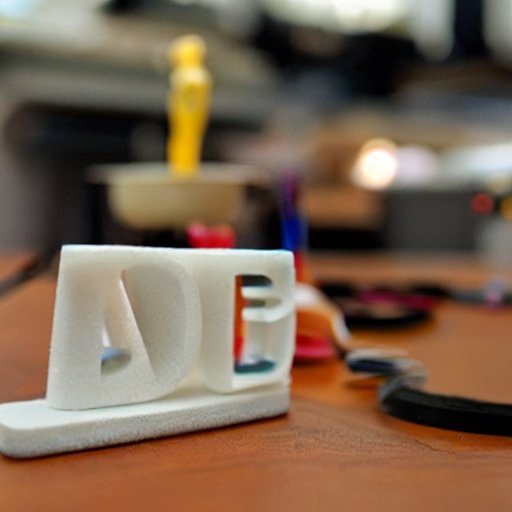
\includegraphics[height=\textheight]{images/replace_me.jpg}}
\end{figure}
\clearpage
%%%%%%%%%%%%%%% end %%%%%%%%%%%%%%%%%%

\LPLsection{Projects}

%%%%%%%%% New content page %%%%%%%%%%%
%%% Bold comment %%%
\noindent {\large \textbf{3D printers are at the heart of LPL}} \\
%%%%%%%%%%%%%%%%%%%%

The assembly of our first FDM 3D printers was one of the first projects at LPL in itself. Today, we have a total of five FDM printers and one SLA printer operational. 
3D printers are at the heart of a prototyping lab because they allow for the rapid creation of physical models and prototypes of designs. This can be particularly useful for testing the form, fit, and function of a design before committing to the time and resources to produce the final product. 3D printing also allows for creating complex geometries and custom parts that may be difficult or impossible to manufacture using traditional methods. This can help to speed up the prototyping process and reduce the need for multiple iterations of a design. 

\clearpage
\begin{figure}
    \centering
    \makebox[\textwidth]{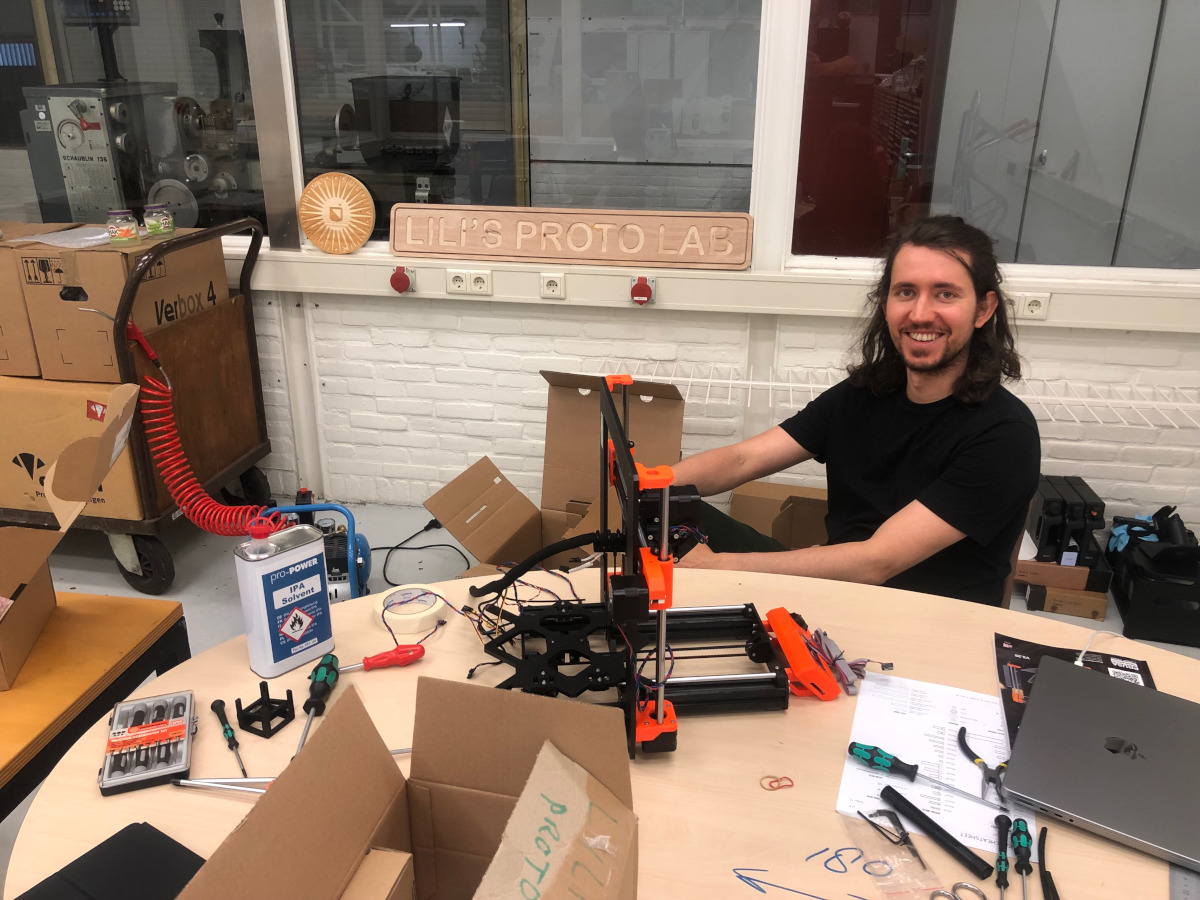
\includegraphics[height=\textheight]{images/prusa_session.jpg}}
\end{figure}
\clearpage
%%%%%%%%%%%%%%% end %%%%%%%%%%%%%%%%%%

%%%%%%%%% New content page %%%%%%%%%%%
%%% Bold comment %%%
\noindent {\large \textbf{The first ever prototype}} \\
%%%%%%%%%%%%%%%%%%%%

This cube is our first eye-catcher and promotional material for our new lab. Is is completely 3D-printed using different colored filaments. The photo of Caroline Bleeker has been converted into a height map such that diffuse light shining from the LEDs inside creates a 3-dimensional visual experience. 

The project and STL files can be found here [INSERT JOGL LINK].

\clearpage
\begin{figure}
    \centering
    \makebox[\textwidth]{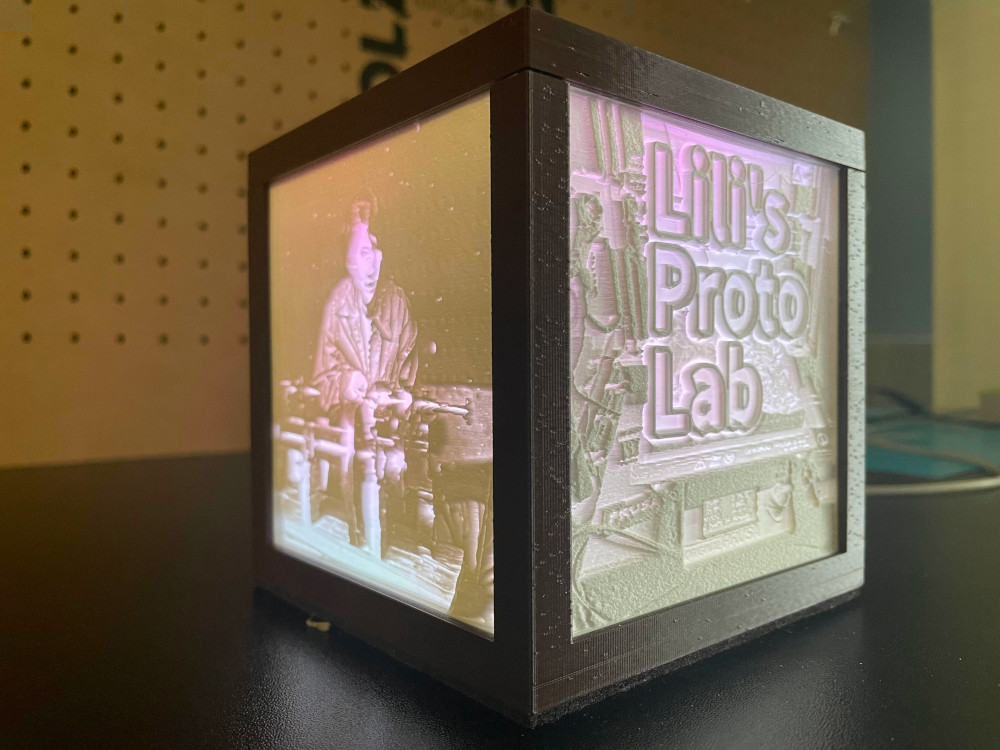
\includegraphics[height=\textheight]{images/cube2.jpg}}
\end{figure}
\clearpage
%%%%%%%%%%%%%%% end %%%%%%%%%%%%%%%%%%%

%%%%%%%%% New content page %%%%%%%%%%%
%%% Bold comment %%%
\noindent {\large \textbf{Edward joins LPL with a chess board project}} \\
%%%%%%%%%%%%%%%%%%%%

The chessboard combines the use of three different tools (and, thus, was a creative leap for Edward to start as a new member of LPL): 1. The AR-shaper for drilling the wood and producing the white chessboard fields, 2. The laser cutter to engrace the black fields, and 3. the 3D printers to print the chess pieces.

The project and STL files can be found here [INSERT JOGL LINK].

\clearpage
\begin{figure}
    \centering
    \makebox[\textwidth]{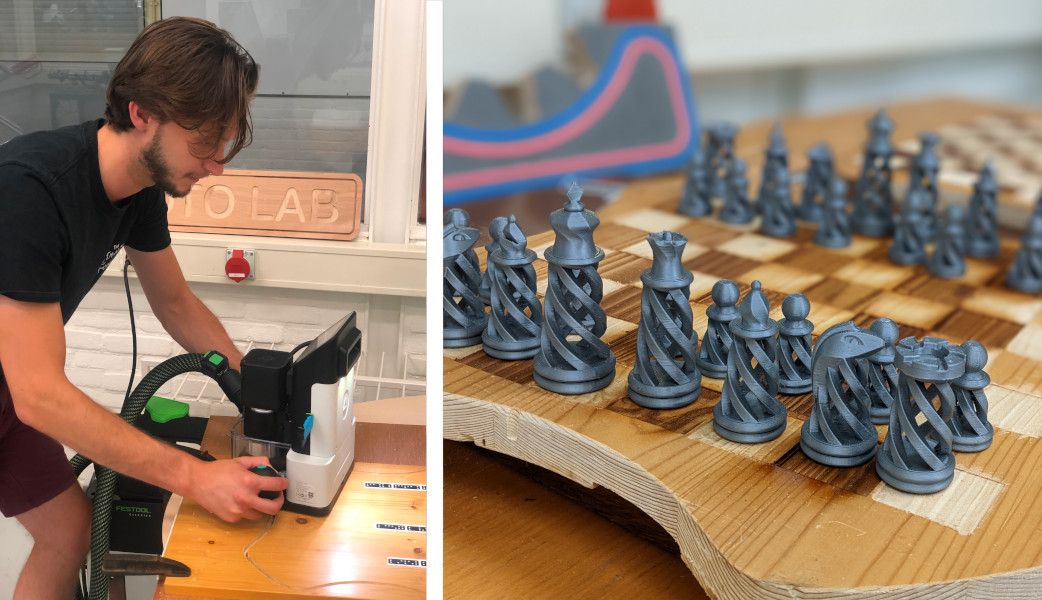
\includegraphics[height=0.85\textheight]{images/chess.jpg}}
\end{figure}
\clearpage
%%%%%%%%%%%%%%% end %%%%%%%%%%%%%%%%%%%

%%%%%%%%% New content page %%%%%%%%%%%
%%% Bold comment %%%
\noindent {\large \textbf{Present for the vice dean}} \\
%%%%%%%%%%%%%%%%%%%%

Education works best when all the parts are working! We hope the vice dean feels inspired by our present to make all gears turn smoothly. 

For this design, we used the Shaper wood drill and laser cutter to cut and engrave the plexiglass. In the bottom of the wood a strip of LEDs is mounted.
The project and SVG file can be found on JOGL:\\
\url{https://app.jogl.io/post/2895}.

\clearpage
\begin{figure}
    \centering
    \makebox[\textwidth]{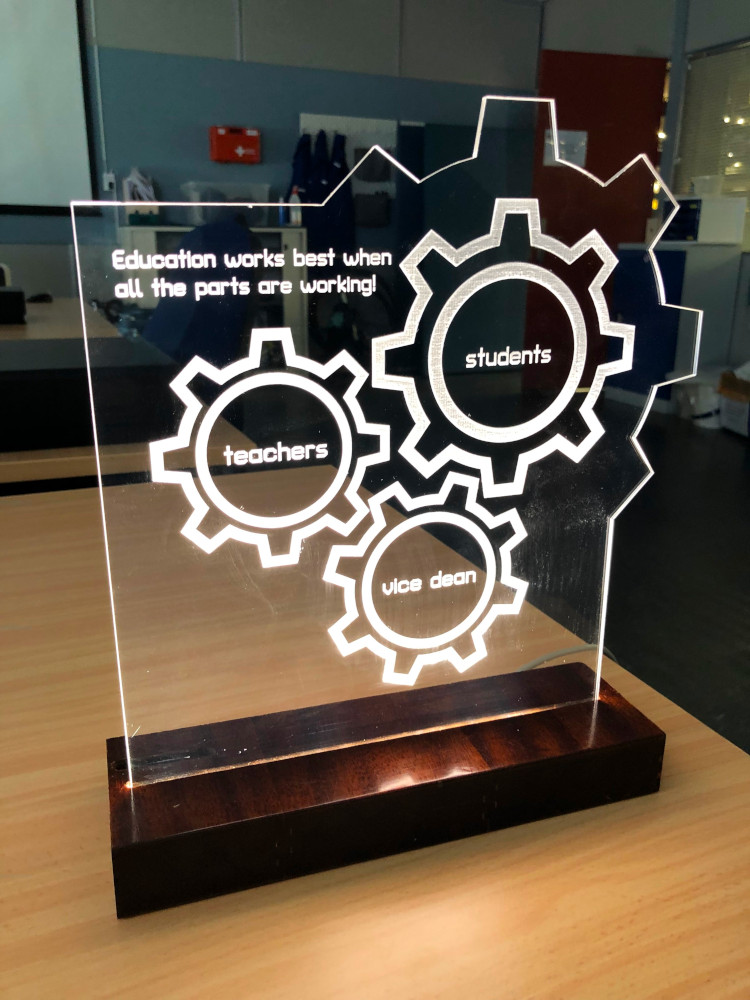
\includegraphics[height=1\textheight]{images/vice_dean.jpg}}
\end{figure}
\clearpage
%%%%%%%%%%%%%%% end %%%%%%%%%%%%%%%%%%%

%%%%%%%%% New content page %%%%%%%%%%%
%%% Bold comment %%%
\noindent {\large \textbf{Award for the bio-inspired design challenge}} \\
%%%%%%%%%%%%%%%%%%%%

The bio-design students who used Lili's Proto Lab won the Bio-inspired design challenge. Here is a photo of them with the award we built. Credit to Nico and Pieter for doing the electronics, and thanks again to Lennart for supplying the LEDs.

The SVG file can be found on JOGL:\\
\url{https://app.jogl.io/post/2896}.

\clearpage
\begin{figure}
    \centering
    \makebox[\textwidth]{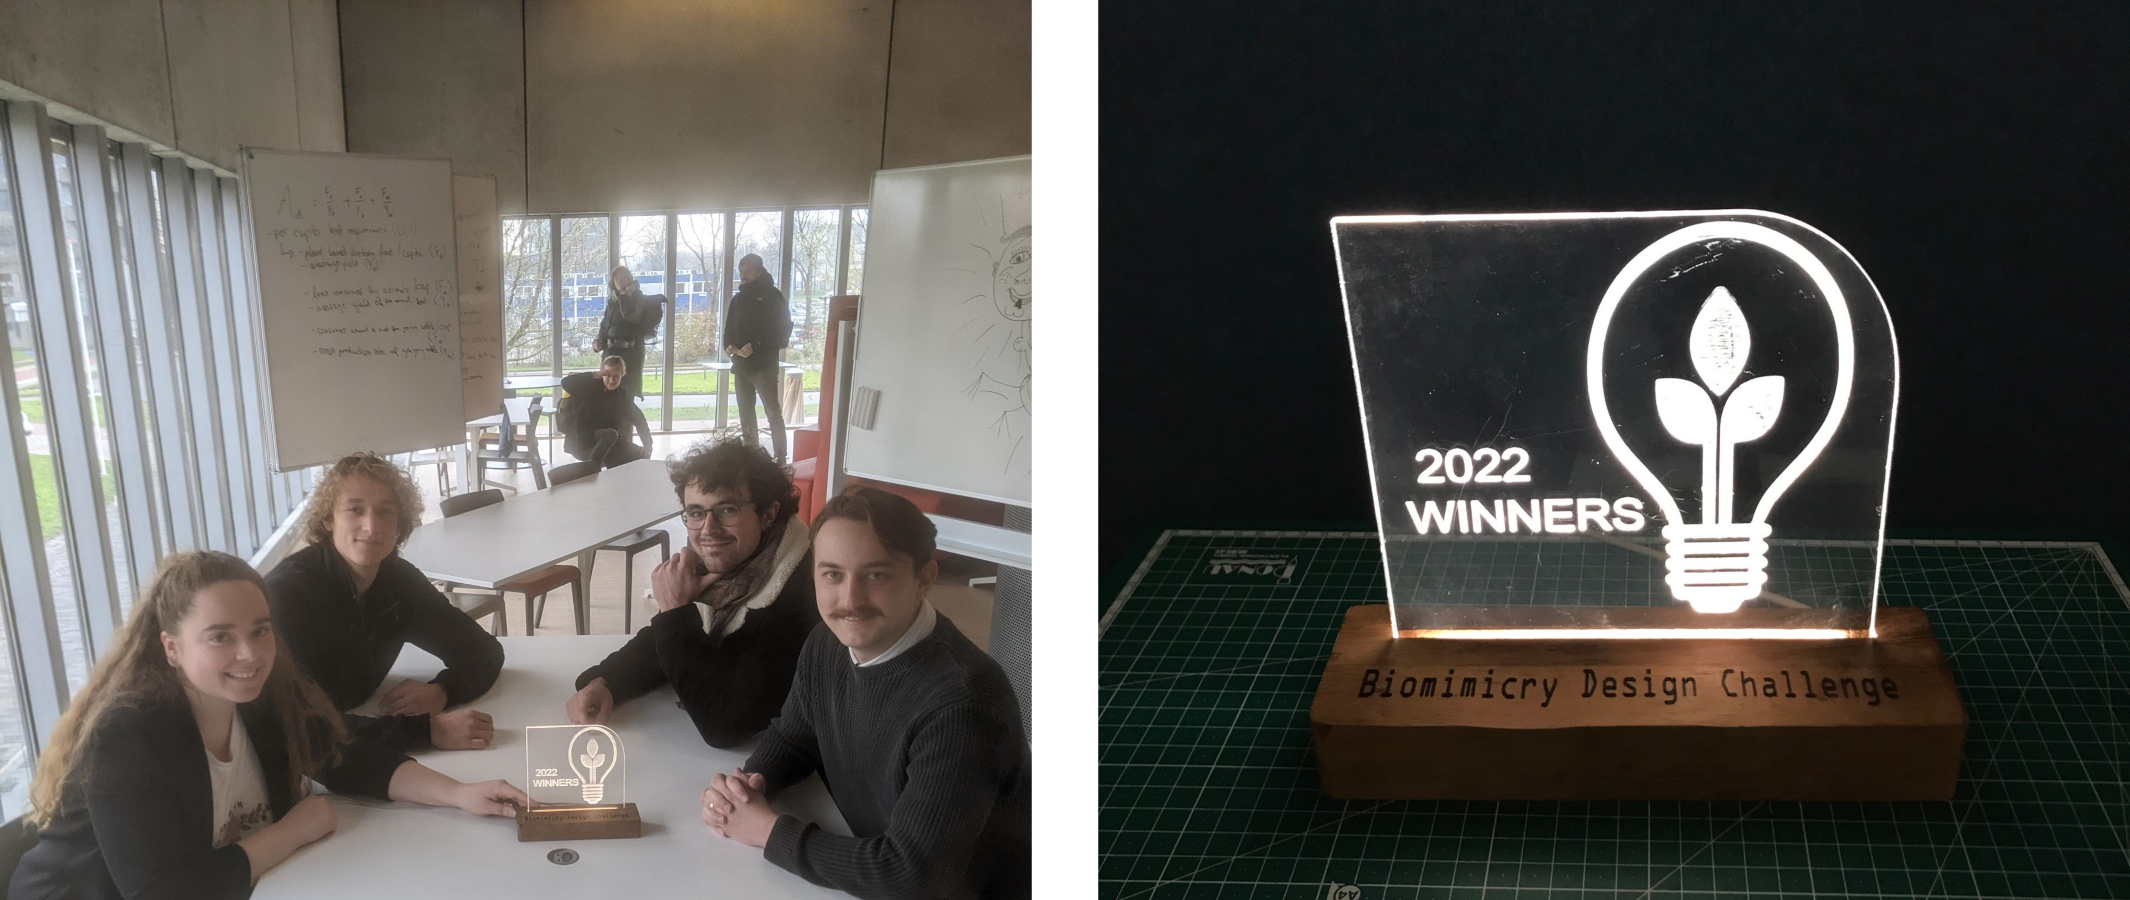
\includegraphics[height=0.7\textheight]{images/bio_design_award.png}}
\end{figure}
\clearpage
%%%%%%%%%%%%%%% end %%%%%%%%%%%%%%%%%%%

%%%%%%%%% New content page %%%%%%%%%%%
%%% Bold comment %%%
\noindent {\large \textbf{Whale Fin}} \\
%%%%%%%%%%%%%%%%%%%%

The 3D whale fin is a project by Menno Bas, a student from the
BioInspired Innovation track. His prototype uses a whale fin shape to
create flow in a fish farming basin with minimal turbulence. At LPL, he
used the vacuum former and laser cutter to create two opposing HIPS
molds from a clay model, from which he cast a 3D silicone rubber fin
prototype.

\clearpage
\begin{figure}
    \centering
    \makebox[\textwidth]{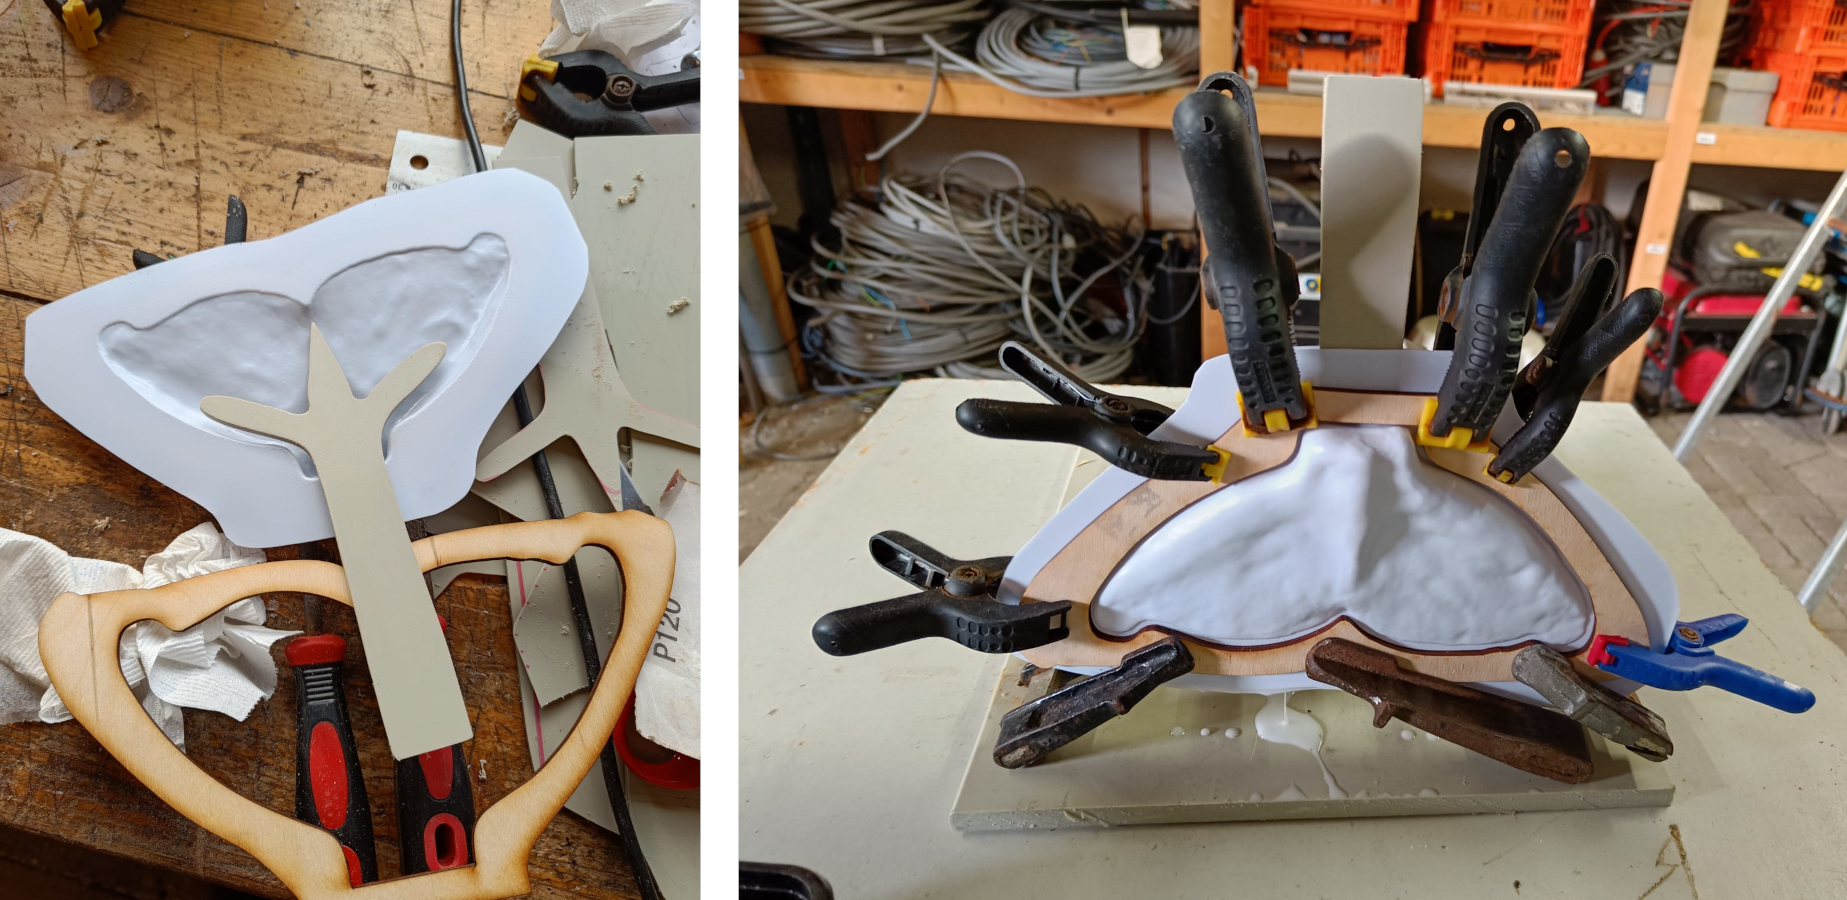
\includegraphics[height=0.8\textheight]{images/whale_fin.png}}
\end{figure}
\clearpage
%%%%%%%%%%%%%%% end %%%%%%%%%%%%%%%%%%%

%%%%%%%%% New content page %%%%%%%%%%%
%%% Bold comment %%%
\noindent {\large \textbf{Detecting particle distributions using light and AI}} \\
%%%%%%%%%%%%%%%%%%%%

Jacob and Lotte are prototyping an optical particle detector for nanosized particles in water. For that, they are building a dark field microscope and a data-driven pipeline to infer individual particle sizes using a deep neural network. The goal is to quantify the particle size distribution and exploit the fact that the astigmatic point-spread function of the microscope can be used to decode spatial information for each particle. \\

This project is documented on JOGL for further reading or contribution:
\url{https://app.jogl.io/project/1176/ParticleDetector}.

\clearpage
\begin{figure}
    \centering
    \makebox[\textwidth]{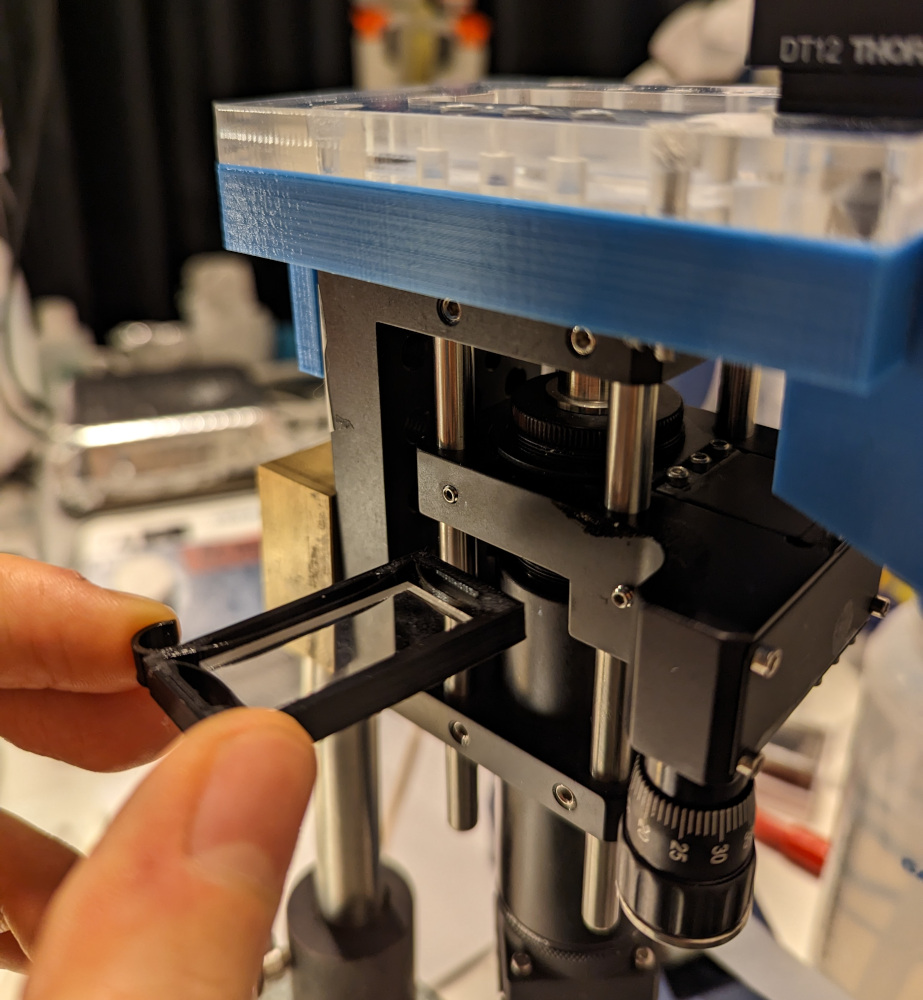
\includegraphics[height=1.0\textheight]{images/particle_detector.jpg}}
\end{figure}
\clearpage
%%%%%%%%%%%%%%% end %%%%%%%%%%%%%%%%%%%

\LPLsection{Supplementary}

%%%%%%%%% New content page %%%%%%%%%%%
%%% Bold comment %%%
\noindent {\large \textbf{List of events}} \\
%%%%%%%%%%%%%%%%%%%%

05.07.2022, Faculty Day, lasercutting workshop\\
25.07.2022, Prusa 3D printer assembly session\\
03.11.2022, Presentations of \textit{Experimental Design} prototypes\\
23.11.2022, LPL advisory board meeting\\
20.12.2022, UU-employee labtour to HCC and LPL\\

\clearpage
\begin{figure}
    \centering
    \makebox[\textwidth]{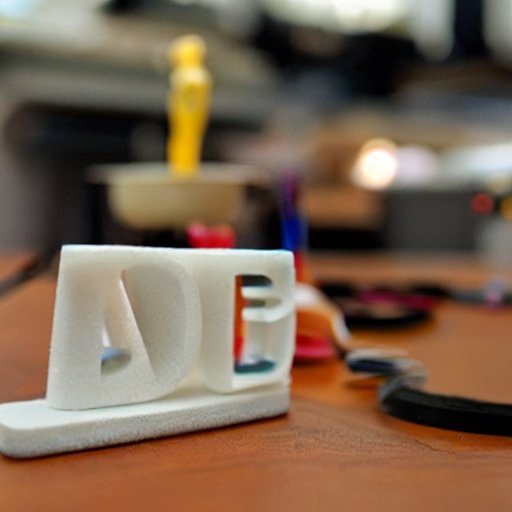
\includegraphics[height=1.0\textheight]{images/replace_me.jpg}}
\end{figure}
\clearpage
%%%%%%%%%%%%%%% end %%%%%%%%%%%%%%%%%%%

%%%%%%%%% New content page %%%%%%%%%%%
%%% Bold comment %%%
\noindent {\large \textbf{Thanks to...}} \\
%%%%%%%%%%%%%%%%%%%%

(List of names who we want to thank. Please fill in more names)\\

Dante Killian, Lotte Polling, Nico van Hijningen, CMD maker space at HU, Annemiek Pronk, Sigrid Jansen, Willem Huijgens, Irma Vermeend, Otto van de Beek, Stefan Vandoren, Han Wosten, Sander Deelen, Rens Voesenek, Ard Spidsbaard, Klaas Druijff, Judith Masthoff, FSC Utrecht University, Christina Verver van Ek, Margot Koster, Peter van der Straten, Quinten Kleijnen, Henk-Jan Akkerman, Hannah Moespot, Lisa van Dijk, 

\clearpage
\begin{figure}
    \centering
    \makebox[\textwidth]{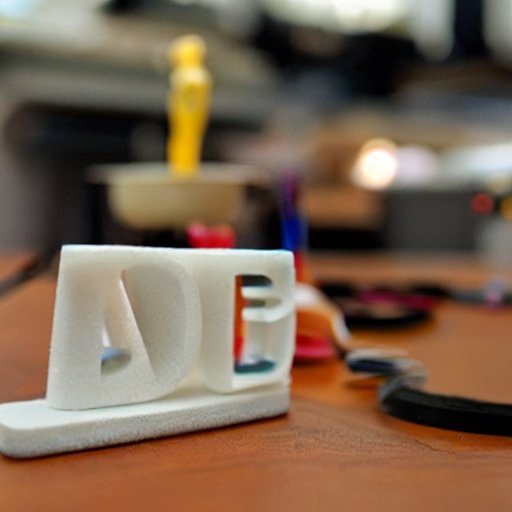
\includegraphics[height=1.0\textheight]{images/replace_me.jpg}}
\end{figure}
\clearpage
%%%%%%%%%%%%%%% end %%%%%%%%%%%%%%%%%%%

\end{document}
